\documentclass[11pt]{article}
\usepackage[utf8]{inputenc}
\usepackage{enumitem}
\usepackage{tikz}
\usepackage{pgf-pie}

\newtheorem{remark}{Disadvantage}
\newtheorem{definition}{Definition}
\newtheorem{prof}{Advantage}

\title{CodeMR Software Metrics Tool}
\author{Alexandru Stoica}
\date{March 2019}

\begin{document}

\maketitle

\section{Introduction}
\texttt{CodeMR} is a software quality and static code analysis tool that helps software companies developing better code, better quality. \texttt{CodeMR} supports multiple programming languages such as Java, Kotlin Scala and C++.

\section{Results}

\begin{center}
\begin{table}[h]
\begin{tabular}{|l|c|}
\hline
Data                                 & Value \\ \hline
lines of code                        & 880   \\ \hline
number of classes                    & 55    \\ \hline
number of packages                   & 9     \\ \hline
number of external packages          & 50    \\ \hline
number of external classes           & 120   \\ \hline
number of problematic classes        & 2     \\ \hline
number of highly problematic classes & 0     \\ \hline
\end{tabular}
\end{table}
\end{center}

\subsection{Complexity}

\begin{definition}
Complexity implies being difficult to understand and describes the interactions between a number of entities. Higher levels of complexity in software increase the risk of unintentionally interfering with interactions and so increases the chance of introducing defects when making changes.
\end{definition}

\begin{center}
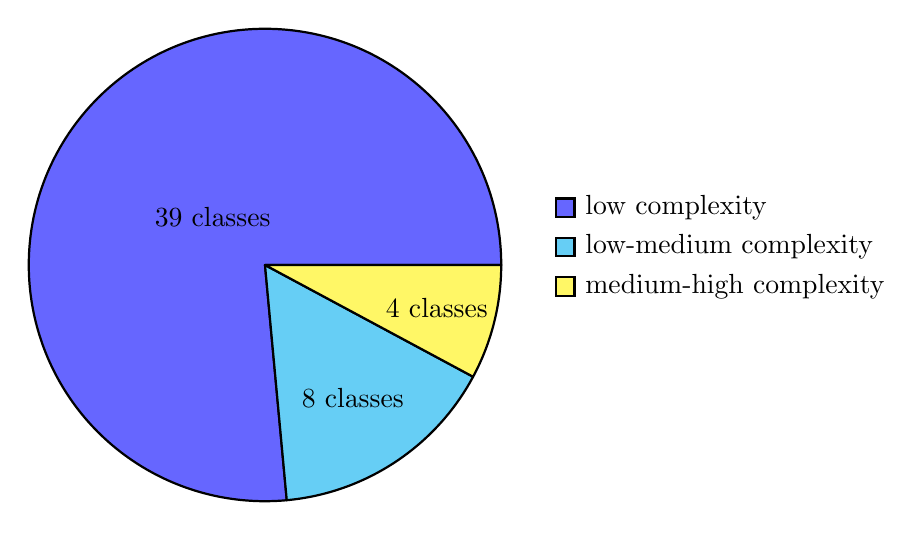
\begin{tikzpicture}
  \pie[sum = auto, text = legend, after number ={ classes} ]{
  39/low complexity,
  8/low-medium complexity,
  4/medium-high complexity
 }
 
\end{tikzpicture}

\textbf{Problem Files:} \\
\texttt{/security/JsonWebTokenAuthenticationFilter.kt} \\
\texttt{/security/JsonWebTokenAuthorizationFilter.kt} \\
\texttt{/report/ReportNotFound.kt} \\
\texttt{/report/UserNotFound.kt}

\end{center}

\subsection{Coupling}

Coupling between two classes A and B if:

\begin{itemize}
  \setlength\itemsep{0.1em}
    \item A has an attribute that refers to (is of type) B.
    \item A calls on services of an object B.
    \item A has a method that references B (via return type or parameter).
    \item A has a local variable which type is class B.
    \item A is a subclass of (or implements) class B.
\end{itemize}

\begin{center}
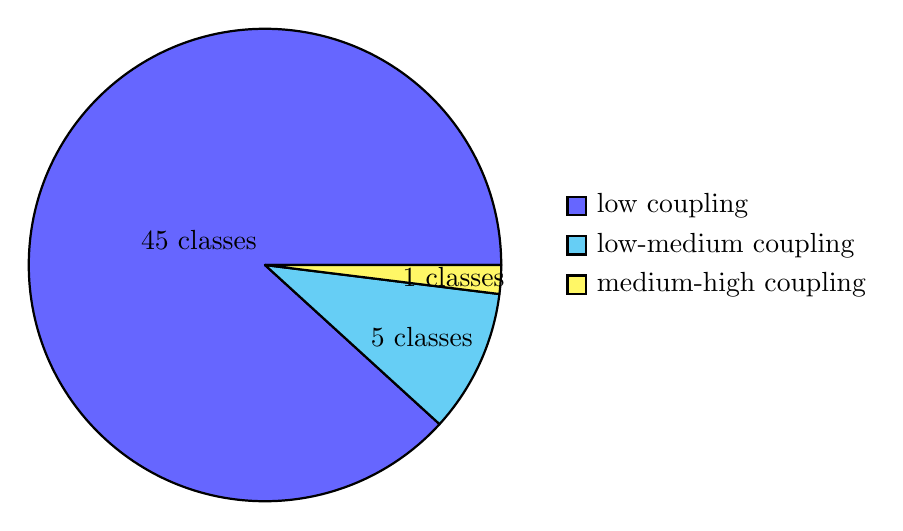
\begin{tikzpicture}
  \pie[sum = auto, text = legend, after number ={ classes} ]{
  45/low coupling,
  5/low-medium coupling,
  1/medium-high coupling
 }
 \end{tikzpicture}

\textbf{Problem Files:} \\
\texttt{/notification/NotificationAspect.kt} \\
\end{center}

Tightly coupled systems tend to exhibit the following characteristics:
\begin{itemize}
  \setlength\itemsep{0.1em}
    \item A change in a class usually forces a ripple effect of changes in other classes.
    \item Require more effort and/or time due to the increased dependency.
    \item Might be harder to reuse a class because dependent classes must be included.
\end{itemize}

\subsection{Lack of Cohesion}


\begin{definition}
\textbf{Lack of cohesion} measures how well the methods of a class are related to each other. 
\end{definition}

High cohesion (low lack of cohesion) tend to be preferable, because high cohesion is associated with several desirable traits of software including robustness, reliability, reusability, and understandability. 

In contrast, low cohesion is associated with undesirable traits such as being difficult to maintain, test, reuse, or even understand.

\begin{center}

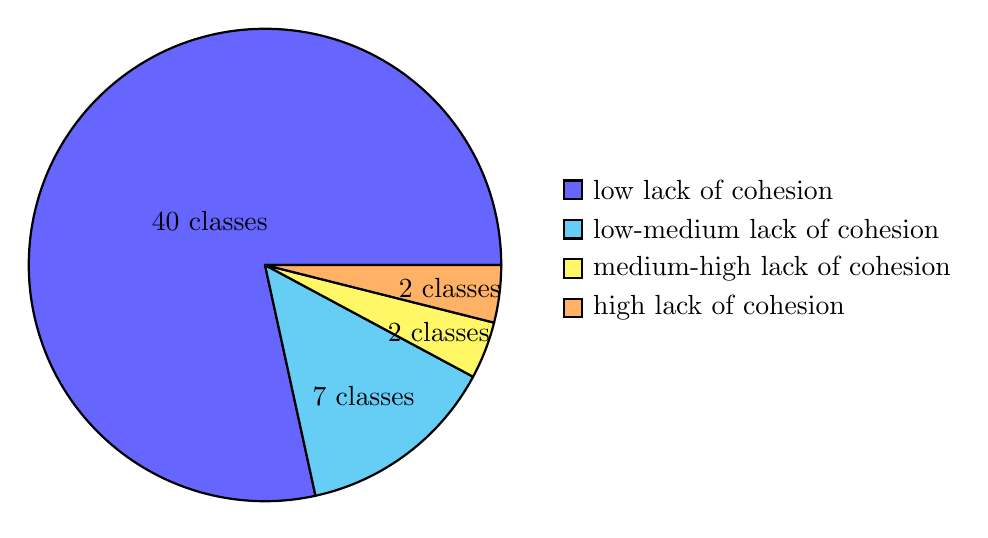
\begin{tikzpicture}
  \pie[sum = auto, text = legend, after number ={ classes} ]{
  40/low lack of cohesion,
  7/low-medium lack of cohesion,
  2/medium-high lack of cohesion,
  2/high lack of cohesion
}
\end{tikzpicture}

\textbf{Problem Files:} \\
\texttt{/user/User.kt} \\
\texttt{/report/Report.kt} \\
\end{center}


\subsection{Size}
\begin{definition}
\textbf{Size} is one of the oldest and most common forms of software measurement. Measured by the number of lines or methods in the code. 
\end{definition}

A very high count might indicate that a class or method is trying to do too much work and should be split up. It might also indicate that the class might be hard to maintain.

\begin{center}
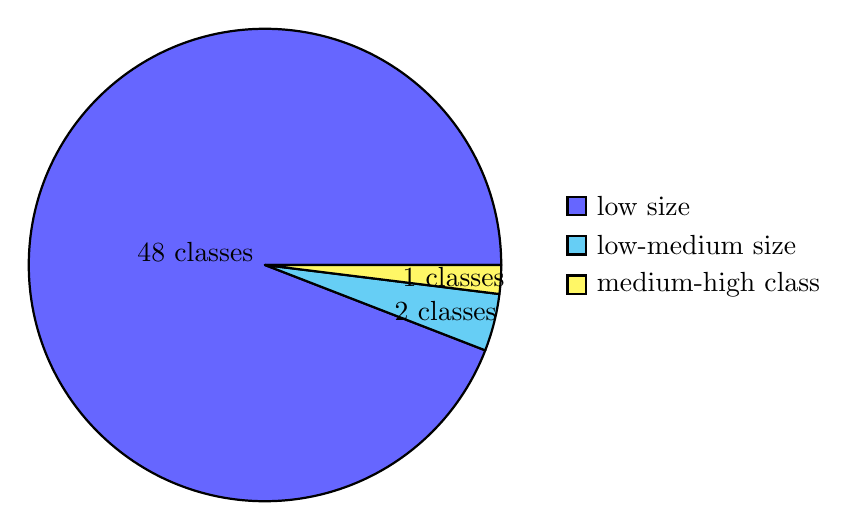
\begin{tikzpicture}
  \pie[
  sum = auto, text = legend, 
  after number ={ classes} ]{
  48/low size,
  2/low-medium size,
  1/medium-high class
}
\end{tikzpicture}

\textbf{Problem Files:} \\
\texttt{/user/User.kt} \\
\end{center}

\subsection{Depth of Inheritance Tree}

Related Quality Attributes: Complexity

\begin{definition}
Depth of inheritance tree represents the position of the class in the inheritance tree. Has 0 (zero) value for root and non-inherited classes.For the multiple inheritance, the metric shows the maximum length. 
\end{definition}

Deeper class in the inheritance tree, probably inherit. Therefore, it is harder to predict its behaviour. Also this class relatively complex to develop, test and maintain.

\begin{center}
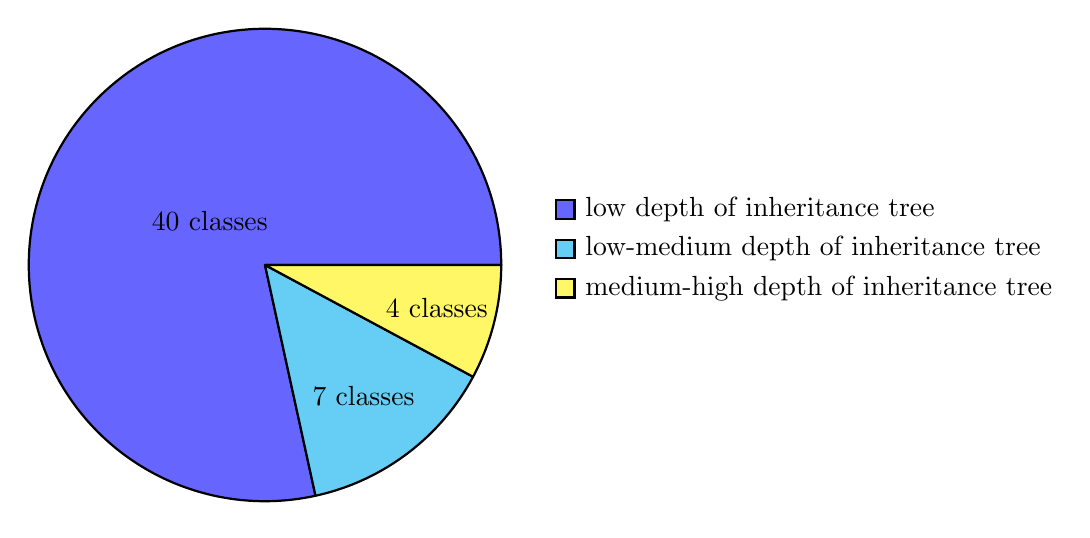
\begin{tikzpicture}
  \pie[
  sum = auto, text = legend, 
  after number ={ classes} ]{
  40/low depth of inheritance tree,
  7/low-medium depth of inheritance tree,
  4/medium-high depth of inheritance tree
}
\end{tikzpicture}

\textbf{Problem Files:} \\
\texttt{/security/JsonWebTokenAuthenticationFilter.kt} \\
\texttt{/security/JsonWebTokenAuthorizationFilter.kt} \\
\texttt{/report/ReportNotFound.kt} \\
\texttt{/user/UserNotFound.kt} \\
\end{center}

\section{Advantages}

\begin{prof}
CodeMR provides intuitive diagrams which show the connections between packages. This feature helps us identify hard-coded dependances (relationships based on concrete classes with no abstraction between the endpoints) between different systems within our application.
\end{prof}

\begin{prof}
Support for Java, Kotlin and Scala all in one package; in today's applications, we require tools able to support various related programming languages since most of our codebases use at least two of them.
\end{prof}

\begin{prof}
CodeMR presents useful diagrams of the codebase's structure, based on projects, packages and classes; this feature helps us examine our code from several perspectives and identify predicaments with ease.
\end{prof}

\section{Disadvantages}

\begin{remark}
The lack of customisation may be CodeMR's weakest spot. Although our engine supports the most commonly calculated metrics such as complexity, lack of cohesion and others, developers are unable to create plugins or extensions to measure additional software quality metrics.
\end{remark} 

\end{document}
